\documentclass[manuscript]{acmart}\usepackage[]{graphicx}\usepackage[]{color}
% maxwidth is the original width if it is less than linewidth
% otherwise use linewidth (to make sure the graphics do not exceed the margin)
\makeatletter
\def\maxwidth{ %
  \ifdim\Gin@nat@width>\linewidth
    \linewidth
  \else
    \Gin@nat@width
  \fi
}
\makeatother

\definecolor{fgcolor}{rgb}{0.345, 0.345, 0.345}
\newcommand{\hlnum}[1]{\textcolor[rgb]{0.686,0.059,0.569}{#1}}%
\newcommand{\hlstr}[1]{\textcolor[rgb]{0.192,0.494,0.8}{#1}}%
\newcommand{\hlcom}[1]{\textcolor[rgb]{0.678,0.584,0.686}{\textit{#1}}}%
\newcommand{\hlopt}[1]{\textcolor[rgb]{0,0,0}{#1}}%
\newcommand{\hlstd}[1]{\textcolor[rgb]{0.345,0.345,0.345}{#1}}%
\newcommand{\hlkwa}[1]{\textcolor[rgb]{0.161,0.373,0.58}{\textbf{#1}}}%
\newcommand{\hlkwb}[1]{\textcolor[rgb]{0.69,0.353,0.396}{#1}}%
\newcommand{\hlkwc}[1]{\textcolor[rgb]{0.333,0.667,0.333}{#1}}%
\newcommand{\hlkwd}[1]{\textcolor[rgb]{0.737,0.353,0.396}{\textbf{#1}}}%
\let\hlipl\hlkwb

\usepackage{framed}
\makeatletter
\newenvironment{kframe}{%
 \def\at@end@of@kframe{}%
 \ifinner\ifhmode%
  \def\at@end@of@kframe{\end{minipage}}%
  \begin{minipage}{\columnwidth}%
 \fi\fi%
 \def\FrameCommand##1{\hskip\@totalleftmargin \hskip-\fboxsep
 \colorbox{shadecolor}{##1}\hskip-\fboxsep
     % There is no \\@totalrightmargin, so:
     \hskip-\linewidth \hskip-\@totalleftmargin \hskip\columnwidth}%
 \MakeFramed {\advance\hsize-\width
   \@totalleftmargin\z@ \linewidth\hsize
   \@setminipage}}%
 {\par\unskip\endMakeFramed%
 \at@end@of@kframe}
\makeatother

\definecolor{shadecolor}{rgb}{.97, .97, .97}
\definecolor{messagecolor}{rgb}{0, 0, 0}
\definecolor{warningcolor}{rgb}{1, 0, 1}
\definecolor{errorcolor}{rgb}{1, 0, 0}
\newenvironment{knitrout}{}{} % an empty environment to be redefined in TeX

\usepackage{alltt}

    \usepackage{rotating}
    \usepackage{tikz}

    %%
    %% \BibTeX command to typeset BibTeX logo in the docs
    \AtBeginDocument{%
      \providecommand\BibTeX{{%
        \normalfont B\kern-0.5em{\scshape i\kern-0.25em b}\kern-0.8em\TeX}}}
    
    %% Rights management information.  This information is sent to you
    %% when you complete the rights form.  These commands have SAMPLE
    %% values in them; it is your responsibility as an author to replace
    %% the commands and values with those provided to you when you
    %% complete the rights form.
    \setcopyright{acmcopyright}
    \copyrightyear{2018}
    \acmYear{2018}
    \acmDOI{10.1145/1122445.1122456}
    
    %% These commands are for a PROCEEDINGS abstract or paper.
    \acmConference[Woodstock '18]{Woodstock '18: ACM Symposium on Neural
      Gaze Detection}{June 03--05, 2018}{Woodstock, NY}
    \acmBooktitle{Woodstock '18: ACM Symposium on Neural Gaze Detection,
      June 03--05, 2018, Woodstock, NY}
    \acmPrice{15.00}
    \acmISBN{978-1-4503-XXXX-X/18/06}
    \usepackage{xcolor}
    
    \definecolor{mutualism}{HTML}{5f8dd3}
    \definecolor{competition}{HTML}{ffcc84}
    %% Submission ID.
    %% Use this when submitting an article to a sponsored event. You'll
    %% receive a unique submission ID from the organizers
    %% of the event, and this ID should be used as the parameter to this command.
    %%\acmSubmissionID{123-A56-BU3}
    
    %%
    %% The majority of ACM publications use numbered citations and
    %% references.  The command \citestyle{authoryear} switches to the
    %% "author year" style.
    %%
    %% If you are preparing content for an event
    %% sponsored by ACM SIGGRAPH, you must use the "author year" style of
    %% citations and references.
    %% Uncommenting
    %% the next command will enable that style.
    %%\citestyle{acmauthoryear}
    
    \usepackage{subfig}
    \title[Supplementary Material for ``Modeling ecological relationships'']{Supplementary Material for ``Modeling competitive and complementary ecological relationships between online communities''}

    %%
    %% end of the preamble, start of the body of the document source.
\IfFileExists{upquote.sty}{\usepackage{upquote}}{}
\begin{document}
    
    %%
    %% The "title" command has an optional parameter,
    %% allowing the author to define a "short title" to be used in page headers.

    
    \maketitle

    \section{Clustering Selection}


    \begin{table}[b]
      \begin{tabular}{c c c}
        Algorithm & Parameter & Values \\ \hline
        All & LSI dimensions $k$ & 10,50,100,200,300,400,500,600,700,850 \\
        HDBSCAN & minimum\_ cluster\_size & 2 \\
        HDBSCAN & min\_samples & 2,3,4,5 \\
        HDBSCAN & cluster\_selection\_ epsilon & 0,0.01,0.05,0.1,0.15,0.2 \\
        HDBSCAN & cluster\_selection\_method & eom \\
        Affinity Propagation & damping & 0.5,0.6,0.7,0.8,0.95,0.97,0.99 \\
        Affinity Propagation & preference\_quantile & 0.1,0.3,0.5,0.7,0.9 \\
        Affinity Propagation & convergence\_iters & 15 \\
        \textit{k}-means & max\_iters & 3000 \\
        \textit{k}-means & n\_inits & 3000 \\
        \textit{k}-means & n\_clusters & 100,500,1000,1250,1750,2000 \\
      \end{tabular}
      \end{table}

    Here we provide additional details on our cluster selection procedure.  We test three different algorithms: \textit{k}-means, HDBSCAN, and affinity-propagation clustering.  The table shows the set of parameters that we began testing for each algorithm. We set out to find a clustering that would have the best possible silhouette score given our choice of hyper parametersFor Affinity propagation and \textit{k}-means we use the implementations in \texttt{sklearn}. For HDBSCAN we use the \texttt{hdbscan} python package and set the minimum\_clutser\_size parameter to 2 so that clusters of size 2 can be detected.

      % <<cluster.selection,echo=>>=
      % dfhdbscan <- fread("resources/hdbscan_selection_data.csv",fill=T)
      % dfhdbscan <- dfhdbscan[order(-silhouette_score)][cluster_selection_method =='eom']
      % dfhdbscan <- dfhdbscan[,n_isolates_str:=gsub('[\\[\\]]','',n_isolates,perl=T)]
      % dfhdbscan <- dfhdbscan[,n_isolates_0:=n_isolates_str=='']
      % dfhdbscan <- dfhdbscan[n_isolates_0==T,n_isolates:=0]
      % dfhdbscan <- dfhdbscan[n_isolates_0==F,n_isolates:=as.numeric(n_isolates_str)]
      % dfhdbscan <- dfhdbscan[n_isolates_0==F,n_isolates:=as.numeric(n_isolates_str)]
      % max_isolates <- 5000
      % cluster_size <- 2
      % min_clusters <- 50
      % dfhdbscan <- dfhdbscan[n_isolates_str < max_isolates]
      % dfhdbscan <- dfhdbscan[n_clusters > min_clusters]
      % dfhdbscan <- dfhdbscan[min_cluster_size == cluster_size]
      % tabhead <- 
      % @ 

\clearpage
\section{Forecast plots}

\begin{figure*}[h]
\centering

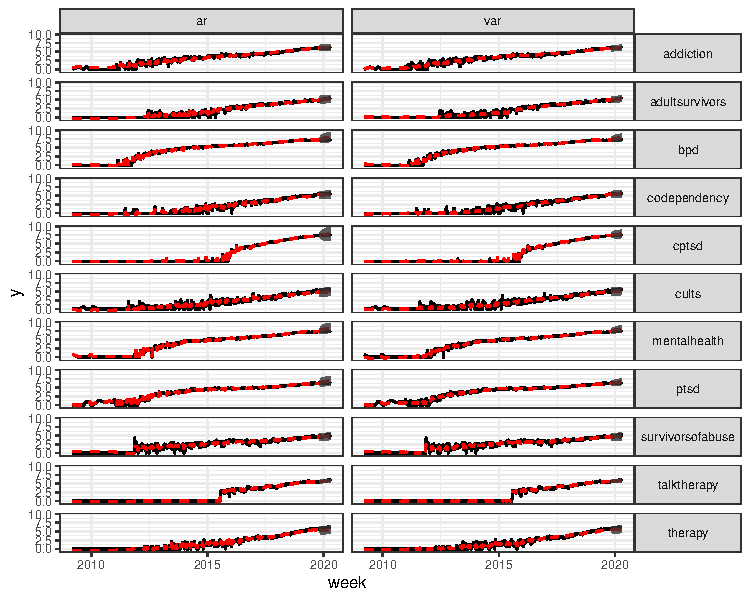
\includegraphics[width=\maxwidth]{figures/knitr-mut_fcast-1} 

\caption{Model fit and forecast from VAR model estimated on cluster of mental health subreddits} 
\end{figure*}

\begin{figure*}
\centering

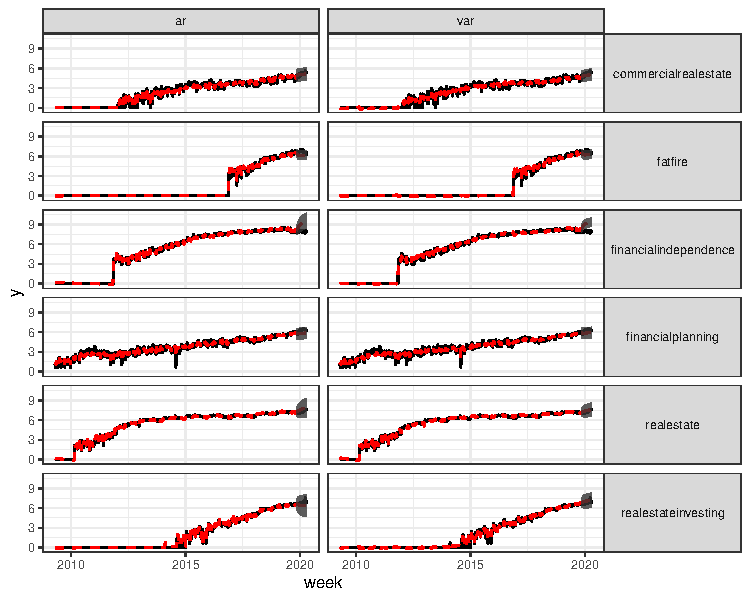
\includegraphics[width=\maxwidth]{figures/knitr-comp_fcast-1} 

\caption{Model fit and forecast from VAR model estimated on cluster of real estate and finance subreddits} 
\end{figure*}

\begin{figure*}
\centering

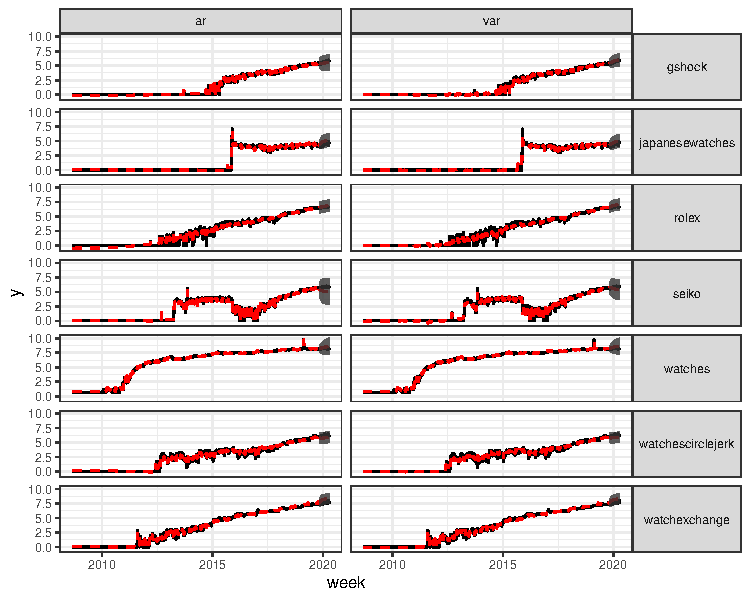
\includegraphics[width=\maxwidth]{figures/knitr-mixed_fcast-1} 

\caption{Model fit and forecast from VAR model estimated on cluster of timepiece subreddits} 
\end{figure*}


\begin{figure*}
\centering

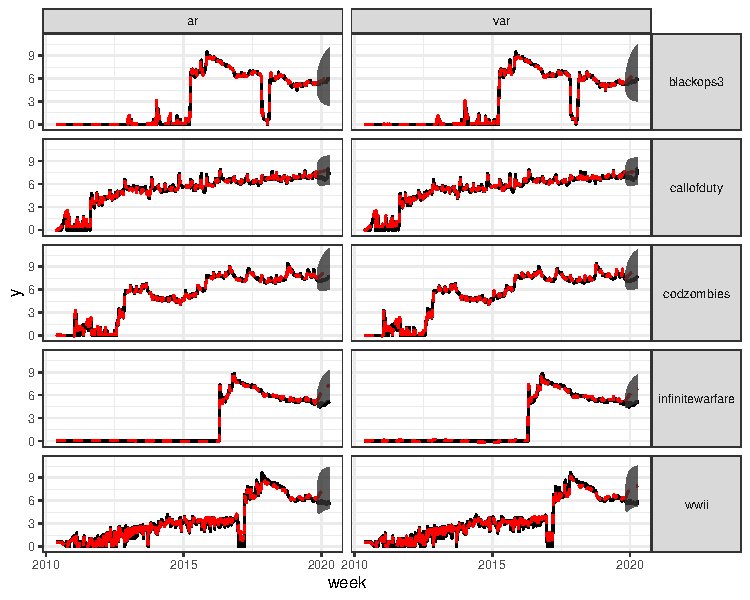
\includegraphics[width=\maxwidth]{figures/knitr-void_fcast-1} 

\caption{Model fit and forecast from VAR model estimated on cluster of call-of-duty subreddits} 
\end{figure*}

\clearpage
\section{Var model coefficients}

\begin{figure*}[h]
\centering

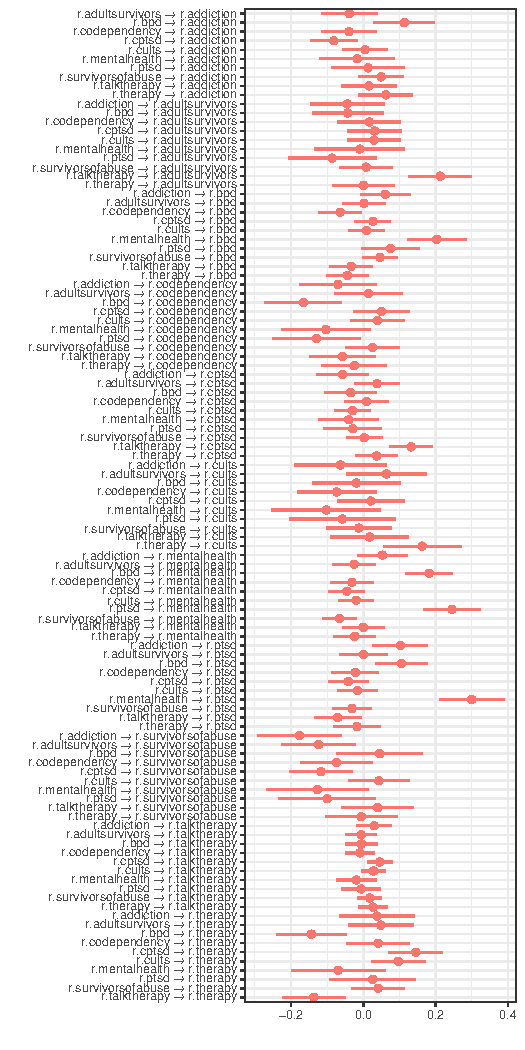
\includegraphics[width=\maxwidth]{figures/knitr-mut_coefs-1} 

\caption{Commensal coefficients from VAR model estimated on cluster of mental health subreddits. \label{mut.coefs}}
\end{figure*}

\begin{figure*}[h]
\centering

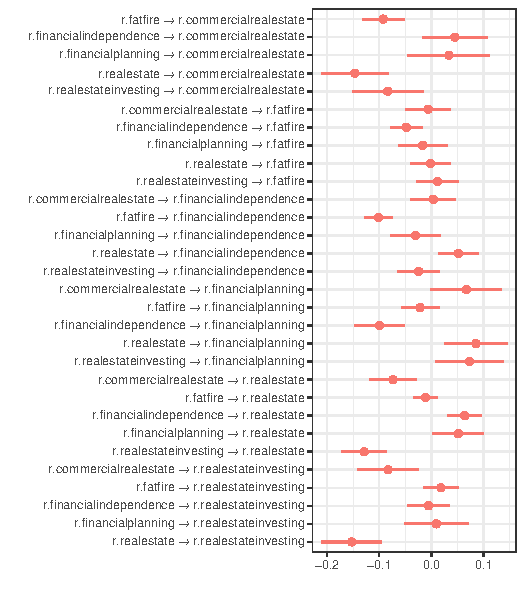
\includegraphics[width=\maxwidth]{figures/knitr-comp_coefs-1} 

\caption{Commensal coefficients from VAR model estimated on cluster of real estate and finance subreddits. \label{comp.coefs}}
\end{figure*}

\begin{figure*}
\centering

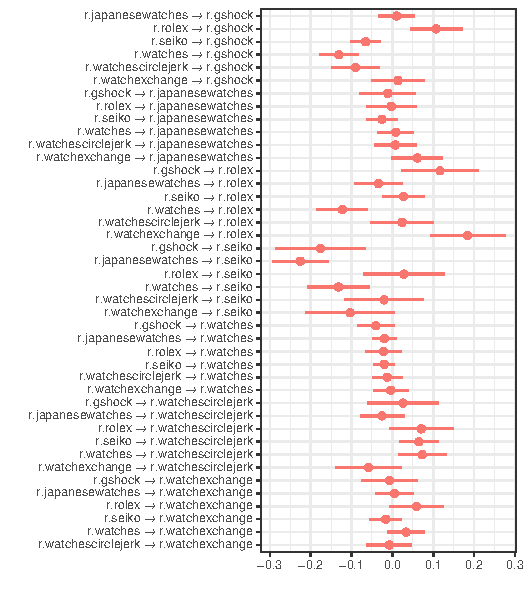
\includegraphics[width=\maxwidth]{figures/knitr-mixed_coefs-1} 

\caption{Commensal coefficients from VAR model estimated on cluster of timepiece subreddits. \label{mixed.coefs}}
\end{figure*}

\begin{figure*}
\centering

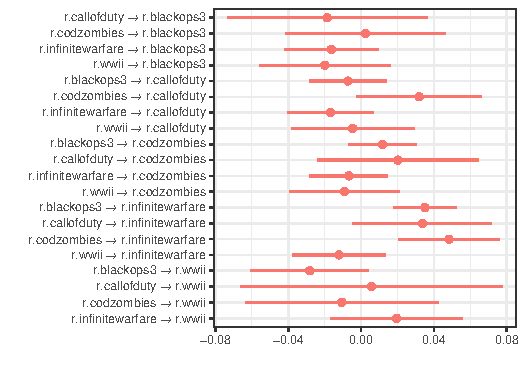
\includegraphics[width=\maxwidth]{figures/knitr-void_coefs-1} 

\caption{Commensal coefficients from VAR model estimated on cluster of art call of duty subreddits. \label{diet.coefs}}
\end{figure*}

\clearpage
\section{Impulse response functions}

\begin{figure*}[h]
\centering

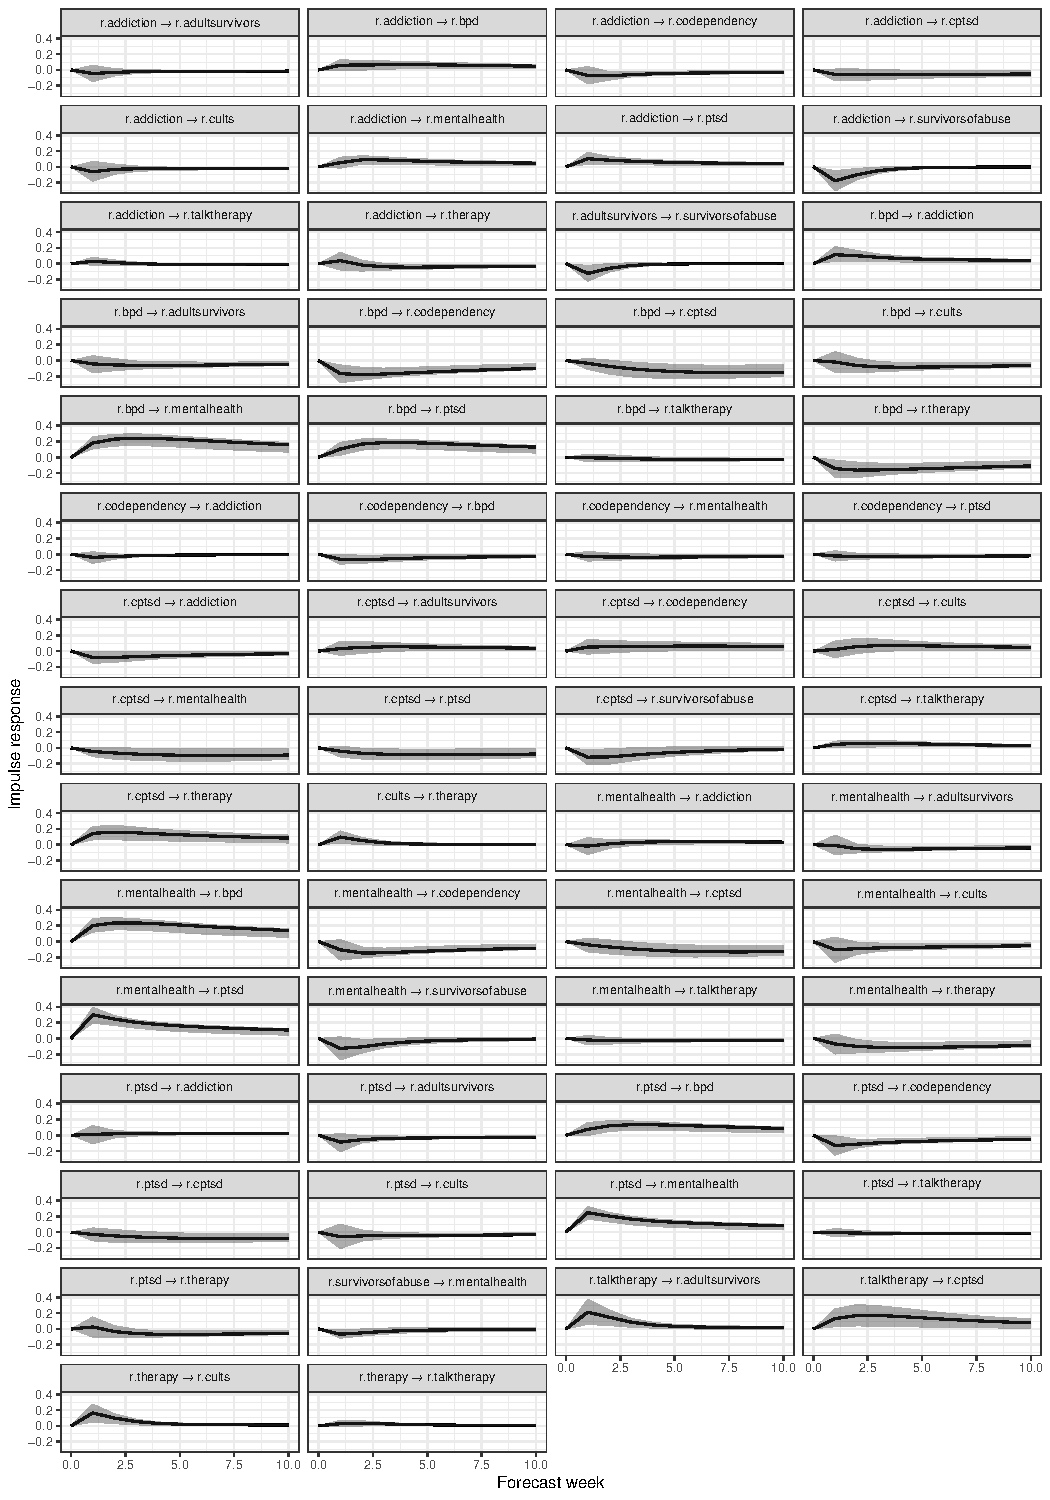
\includegraphics[width=\maxwidth]{figures/knitr-mut_irf-1} 

\caption{Impulse response functions from VAR model estimated on cluster of mental health subreddits. Only impulses where the 95\% confidence interval of the impulse response function does not include 0 are shown. \label{mut.irf}}
\end{figure*}


\begin{figure*}[h]
\centering

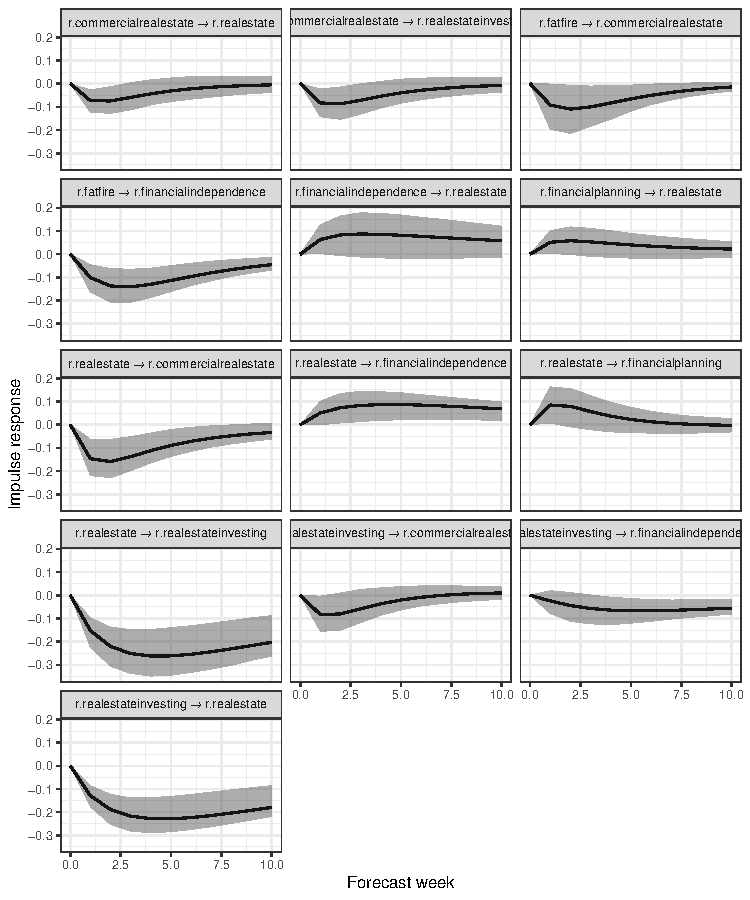
\includegraphics[width=\maxwidth]{figures/knitr-comp_irf-1} 

\caption{Impulse response functions from VAR model estimated on cluster of real estate and finance subreddits. Only impulses where the 95\% confidence interval of the impulse response function does not include 0 are shown. \label{comp.irf}}
\end{figure*}

\begin{figure*}
\centering

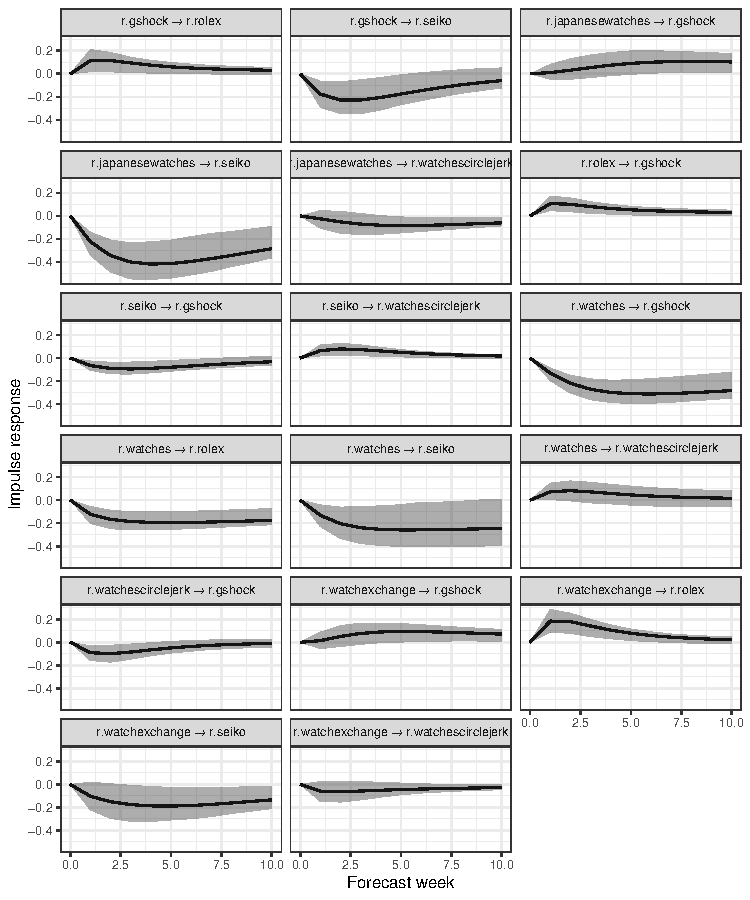
\includegraphics[width=\maxwidth]{figures/knitr-mixed_irf-1} 

\caption{Impulse response functions from VAR model estimated on cluster of timepiece subreddits. Only impulses where the 95\% confidence interval of the impulse response function does not include 0 are shown. \label{mixed.irf}}
\end{figure*}

\begin{figure*}
\centering

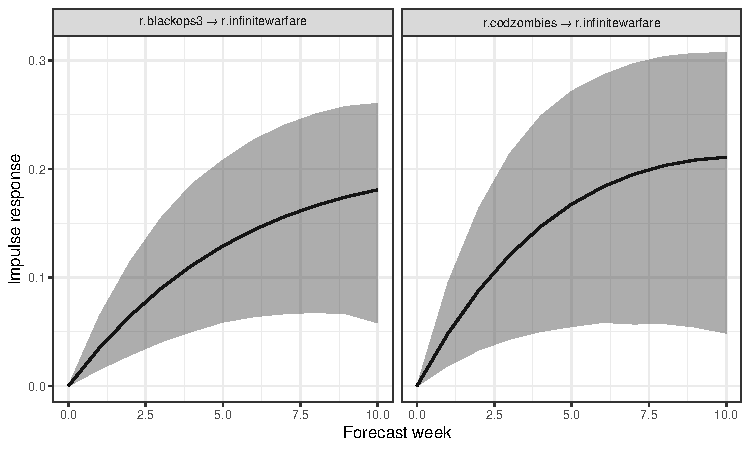
\includegraphics[width=\maxwidth]{figures/knitr-void_irf-1} 

\caption{Impulse response functions from VAR model estimated on cluster of call of duty subreddits. Only impulses where the 95\% confidence interval of the impulse response function does not include 0 are shown. \label{void.irf}}
\end{figure*}

% \begin{figure*}
% \centering
% <<comp.coefs, echo=F, results='asis', fig.width=3.5, fig.height=2.5>>=
% coef <- tanks.var$var.coef.author_cluster_1763_tf
% ctab <- plot.coef.ols.data(coef)

% p <- dwplot(ctab)

% p <- p + scale_y_discrete(labels=parse(text=levels(ctab$term)),breaks=levels(ctab$term))
% print(p)
% @ 
% \caption{Commensal coefficients from VAR model estimated on cluster of toy collection subreddits.}
% \end{figure*}


% \begin{figure*}[t]
% \centering
% <<comp.irf, echo=F, results='asis', fig.width=5, fig.height=3>>=

% irf <- plot.irf.ols.data(tanks.var$irf.ortho.data.author_cluster_1763_tf)

% p <- ggplot(irf,aes(x=x,y=irf,ymax=irf.upper,ymin=irf.lower)) + geom_line() + geom_ribbon(alpha=0.4) + facet_wrap(. ~ facet.title.expr,labeller=label_parsed)

% print(p)
% @ 
% \caption{Impulse response functions from VAR model estimated on cluster of military vehicle subreddits.}
% \end{figure*}


% \subsection{A mixture of competition and mutualism among drawing subreddits}

% \begin{figure*}[t]
% \centering
% <<mixed.coefs, echo=F, results='asis', fig.width=3.5, fig.height=2.5>>=
% coef <- art.var$var.coef.author_cluster_1636_tf
% ctab <- plot.coef.ols.data(coef)

% p <- dwplot(ctab)

% p <- p + scale_y_discrete(labels=parse(text=levels(ctab$term)),breaks=levels(ctab$term))
% print(p)
% @ 

% \caption{Commensal coefficients from VAR model estimated on cluster of drawing subreddits.}
% \end{figure*}


% \begin{figure*}[t]
% \centering
% <<mixed.irf, echo=F, results='asis', fig.width=5, fig.height=3>>=

% irf <- plot.irf.ols.data(art.var$irf.ortho.data.author_cluster_1636_tf)

% p <- ggplot(irf,aes(x=x,y=irf,ymax=irf.upper,ymin=irf.lower)) + geom_line() + geom_ribbon(alpha=0.4) + facet_wrap(. ~ facet.title.expr,labeller=label_parsed)

% print(p)
% @ 
% \caption{Impulse response functions from VAR model estimated on cluster of weight-loss subreddits.}
% \end{figure*}


% \begin{figure*}[t]
% \centering
% <<void.coefs, echo=F, results='asis', fig.width=3.5, fig.height=2.5>>=
% coef <- diet.var$var.coef.author_cluster_1_tf
% ctab <- plot.coef.ols.data(coef)

% p <- dwplot(ctab)

% p <- p + scale_y_discrete(labels=parse(text=levels(ctab$term)),breaks=levels(ctab$term))
% print(p)
% @ 
% \caption{Commensal coefficients from VAR model estimated on cluster of weight-loss subreddits.}
% \end{figure*}


% \begin{figure*}[t]
% \centering
% <<void.irf, echo=F, results='asis', fig.width=5, fig.height=3>>=

% irf <- plot.irf.ols.data(diet.var$irf.ortho.data.author_cluster_1_tf)

% p <- ggplot(irf,aes(x=x,y=irf,ymax=irf.upper,ymin=irf.lower)) + geom_line() + geom_ribbon(alpha=0.4) + facet_wrap(. ~ facet.title.expr,labeller=label_parsed)

% print(p)
% @ 
% \caption{Impulse response functions from VAR model estimated on cluster of weight-loss subreddits.}
% \end{figure*}


% \section{Simulation study}
% Here are results from the simulation study with 6 groups.
% %and from second simulation study with 15 groups.  
% The simulation with 6 groups was designed to represent realistic data with strong commensal relationship. 
% %Parameters in the simulation with 15 groups were randomly generated with a matrix $\Phi$ with real eigenvalues less than,  $\mu$ drawn from a standard normal distribution and $\Sigma$ parameters generated by squaring a matrix drawn from normal distribution with mean 0.2 and variance 0.01 for diagnoal elements and mean 0 and variance 0.01 for off-diagnoal elements.
% \begin{table*}[t]
% \centering
% \subfloat[$\Phi$ parameter in our simulation study representing an ecological community with a variety of commensal relationships.]{
% \label{tab:phi_sim}
% <<show.sim.varmat,results='asis',echo=F>>=

%     obj <- simulated_phi[,,]

%     if(opts_chunk$get("dev") == 'tikz'){
%         names <- sapply(1:dim(obj)[1],function(i) paste0('$y_',i,'$'))
%     } else {
%         names <- sapply(1:dim(obj)[1],function(i) paste0('y',i,''))
%     }

%     colnames(obj) <- names
%     rownames(obj) <- names
%     obj[obj < 0] <- paste0("\\color{competition}",obj[obj < 0])
%     obj[obj > 0] <- paste0("\\color{mutualism}",obj[obj > 0])
%     txt <- xtable(obj,  label='tab:phi_sim',auto=TRUE)
%     align(txt) <- rep('c',ncol(txt)+1)
%     print(txt,type='latex',include.rownames=TRUE,caption.placement='top',floating=FALSE)
% @
% }
%     % txt <- kable(obj, format='latex', booktabs=FALSE, escape=FALSE,
%     % caption="$\\Phi$ parameter in our simulation study representing an ecological community with a variety of commensal relationships.",
%     % label=) 
% \qquad
% \subfloat[Recovered parameters from fitting our model to simulated data.  Highlighted coefficients have 95\% credible intervals that do not include 0.]{
% \label{label='tab:phi_sim_recovered'}
% <<sim.results.varmat, results='asis',echo=F>>=
%     stats <- simulation.phi.stats.95 
%     median <- t(stats$medians[,,])
%     upper <- t(stats$upper[,,])
%     lower <- t(stats$lower[,,])

%     if(opts_chunk$get("dev") == 'tikz'){
%         names <- sapply(1:dim(median)[1],function(i) paste0('$y_',i,'$'))
%     } else {
%         names <- sapply(1:dim(median)[1],function(i) paste0('y',i,''))
%     }

%     sign.neg <- upper < 0
%     sign.pos <- lower > 0
%     obj <- round(median,2)
%     obj[sign.neg] <- paste0("\\color{competition}",obj[sign.neg])
%     obj[sign.pos] <- paste0("\\color{mutualism}",obj[sign.pos])
%     colnames(obj) <- names
%     rownames(obj) <- names

%     txt <- xtable(obj, ,auto=TRUE)
%     align(txt) <- rep('c',ncol(txt)+1)
%     print(txt,type='latex',include.rownames=TRUE,caption.placement='top',floating=FALSE)
% @
% }
% \end{table*}


% \begin{figure*}[h]
% <<sim.irf, fig.env='figure', fig.height=2,echo=F,warning=F>>=
    
%     df <- copy(as.data.table(simulation.irf.forecast.data))
    
%     if(opts_chunk$get("dev") == 'tikz'){
%         df <- df[,name.row := paste0(gsub('y','$y_',name.row),'$')]
%         df <- df[,name.col := paste0(gsub('y','$y_',name.col),'$')]
%         focal.sub <- '$y_1$'

%     } else {
%         focal.sub <- 'y1'
%     }

%     matnames <- unique(df$name.row)

%     level <- '95'

%     if(level=='95')
%         setnames(df,old=c('97.5%','2.5%'),new=c('upper','lower'),skip_absent=T)
%     if(level=='90')
%         setnames(df,old=c('95%','5%'),new=c('upper','lower'),skip_absent=T)
%     if(level=='80')
%         setnames(df,old=c('85%','15%'),new=c('upper','lower'),skip_absent=T)

%     df <- df[(name.row == focal.sub) | (name.col==focal.sub)]
%     df <- df[(name.row != name.col)]

%     if(opts_chunk$get("dev") == 'tikz'){
%         df <- df[,":="(name.row = factor(name.row,levels=matnames),
%                                          name.col = factor(name.col,levels=matnames),
%                                         dir=ifelse(name.row==focal.sub,paste0("$y_m \\rightarrow$ ",focal.sub),paste0(focal.sub,"$ \\rightarrow ","y_m$")),
%                                          name=ifelse(name.row==focal.sub,name.col,name.row)
%                                      )]
%     } else {
%         df <- df[,":="(name.row = factor(name.row,levels=matnames),
%                         name.col = factor(name.col,levels=matnames),
%                         dir=ifelse(name.row==focal.sub,paste0("on ",focal.sub),paste0("of ",focal.sub)),
%                         name=ifelse(name.row==focal.sub,name.col,name.row)
%                 )]
%     }
%     df[['median']] <- df[['50%']]

%     p <- ggplot(df, aes(x=x, y=median, ymin=lower,ymax=upper)) + geom_line() + geom_ribbon(alpha=0.5) + facet_grid(dir~name)
 
%     p <- p + xlim(1,8)
%     p <- p + xlab("Forecast week") + ylab("Impulse response")
%     p

% @
% \caption{Example impulse response functions for $y_1$ from our simulation study}
% \end{figure*}

% \subsection{Large simulation with 15 groups}

% \begin{table*}[t]
% \centering
% \subfloat[$\Phi$ parameter in the large simulation study representing an ecological community with a variety of commensal relationships.]{
% \label{tab:phi_sim}
% <<show.sim.varmat.large,results='asis',echo=F>>=

%     obj <- signif(large_simulated_phi[,,],1)

%     if(opts_chunk$get("dev") == 'tikz'){
%         names <- sapply(1:dim(obj)[1],function(i) paste0('$y_',i,'$'))
%     } else {
%         names <- sapply(1:dim(obj)[1],function(i) paste0('y',i,''))
%     }

%     colnames(obj) <- names
%     rownames(obj) <- names
%     obj[obj < 0] <- paste0("\\color{competition}",obj[obj < 0])
%     obj[obj > 0] <- paste0("\\color{mutualism}",obj[obj > 0])
%     txt <- xtable(obj,  label='tab:phi_sim',auto=TRUE)
%     align(txt) <- rep('c',ncol(txt)+1)
%     print(txt,type='latex',include.rownames=TRUE,caption.placement='top',floating=FALSE)
% @
% }
%     % txt <- kable(obj, format='latex', booktabs=FALSE, escape=FALSE,
%     % caption="$\\Phi$ parameter in our simulation study representing an ecological community with a variety of commensal relationships.",
%     % label=) 

% \caption{True parameters from fitting our model to simulated data.  Highlighted coefficients have 95\% credible intervals that do not include 0.}
% \end{table*}
% \begin{table*}
% <<sim.results.varmat.large, results='asis',echo=F>>=
%     stats <- large_simulation.phi.stats.95 
%     median <- signif((t(stats$medians[,,]),1)
%     upper <- t(stats$upper[,,])
%     lower <- t(stats$lower[,,])

%     if(opts_chunk$get("dev") == 'tikz'){
%         names <- sapply(1:dim(median)[1],function(i) paste0('$y_',i,'$'))
%     } else {
%         names <- sapply(1:dim(median)[1],function(i) paste0('y',i,''))
%     }

%     sign.neg <- upper < 0
%     sign.pos <- lower > 0
%     obj <- round(median,2)
%     obj[sign.neg] <- paste0("\\color{competition}",obj[sign.neg])
%     obj[sign.pos] <- paste0("\\color{mutualism}",obj[sign.pos])
%     colnames(obj) <- names
%     rownames(obj) <- names

%     txt <- xtable(obj, ,auto=TRUE)
%     align(txt) <- rep('c',ncol(txt)+1)
%     print(txt,type='latex',include.rownames=TRUE,caption.placement='top',floating=FALSE)
% @
% \caption{Recovered parameters from fitting our model to simulated data.  Highlighted coefficients have 95\% credible intervals that do not include 0.}

% \end{table*}



% \begin{figure}

% <<large_simulation_coef,results='asis',echo=F,fig.height=9,fig.width="\\textwidth",message=F>>=

%     stats <- copy(large_simulation.phi.stats.95)
%     median <- t(stats$medians[,,])
%     upper <- t(stats$upper[,,])
%     lower <- t(stats$lower[,,])
%     names <- sapply(1:dim(large_simulated_phi)[2],function(i) paste0('Y',i))
%     plot.df <- list()
%     m <- dim(stats$median[,,])[1]#$
%     idx <- 1
%     for(i in 1:m){
%         for(j in 1:m){
%             plot.df[[idx]] <- list('i'=i,'j'=j,'coef'=median[i,j],'upper'=upper[i,j],'lower'=lower[i,j],
%             'true'=large_simulated_phi[,,][i,j],
%             name.expr=paste0(names[[i]],"%->%",names[[j]]),
%             name.tex=paste0(names[[i]],"$\\rightarrow$",names[[j]]))
%             idx <- idx + 1
%         }
%     }
%     plot.df <- rbindlist(plot.df)

%     plot.df <- plot.df[,':='(name.tex = factor(name.tex,levels=rev(name.tex)))]
%     plot.df <- plot.df[,':='(name.expr = factor(name.expr,levels=rev(name.expr)))]

%     if(opts_chunk$get("dev") == 'tikz'){
%         plot.df$name = plot.df$name.tex
%     } else {
%         plot.df$name = plot.df$name.expr
%     }

%     N.sim.wrong <- nrow(plot.df[(true < lower) | (true > upper)])
    
%     p <- plot.coefs(large_simulation.phi.stats.80, names, large_simulation.phi.stats.90, large_simulation.phi.stats.95, stat.names=c("80%","90%","95%"),include.all=T,point.shape.name='estimate',ncols=3)

%     p <-  p + geom_point(aes(x=name,y=true,shape='value'),data=plot.df,size=1.5) + coord_flip()


%     p <- p + scale_shape_manual(name='',values=c(estimate=19,value=1), breaks=c("estimate","value"), labels=c("Estimate","True value"))
%     p <- p + ylab("Value") + xlab("Coefficient") + theme(legend.position='bottom',panel.grid.minor.y=element_blank(),panel.grid.major.y=element_blank())
%     p <- p + scale_x_discrete(labels = parse(text=levels(plot.df$name)))#$
%     p <- p + guides(color=guide_legend(direction='vertical',ncol=2,byrow=F), shape=guide_legend(direction='vertical'))
%     print(p)
% @
% % # p <- p + scale_color_manual(name='',values=c('black','blue'),breaks=c("estimate","value"),labels=c("Estimate","True value"),override.aes=list(color=c('black','blue')))

% \caption{Results of larger simulation with 15 groups study demonstrating that our model can recover true values of $\Phi$ with medians and 95\% credible intervals.  True simulated values are shown in blue and the median and 95\% credible intervals (CI) from our fitted model are shown in black. "}
% \end{figure}

% \clearpage
% \section{Seattle-area case study}
% Here is the full $\Phi$ matrix estimated in our case study of Seattle-area subreddits. 

% \begin{table*}[h]
% \centering
% <<seattle.varmat, results='asis',echo=F>>=
%     stats <- seattle.phi.stats.80
%     median <- t(stats$medians[,,])
%     upper <- t(stats$upper[,,])
%     lower <- t(stats$lower[,,])

%     names <- gsub('_','\\_',unique(seattle.fit.df$subreddit))

%     sign.neg <- upper < 0
%     sign.pos <- lower > 0
%     obj <- round(median,2)
%     obj[sign.neg] <- paste0("\\color{competition}",obj[sign.neg])
%     obj[sign.pos] <- paste0("\\color{mutualism}",obj[sign.pos])
%     colnames(obj) <- names
%     rownames(obj) <- names

%     txt <- xtable(obj, auto=TRUE)
%     align(txt) <- rep('c',ncol(txt)+1)
%     print(txt,type='latex',include.rownames=TRUE,caption.placement='top',floating=FALSE,rotate.colnames=TRUE)
% @
% \caption{Full matrix $\Phi$ for Seattle-area subreddits. Highlighted coefficients have 80\% credible intervals that do not include 0.}
% \end{table*}

% \clearpage


% \begin{figure*}
% \centering

% <<seattle.coefs, echo=F, results='asis',fig.width='\\textwidth',fig.height=9>>=
%     p <- plot.coefs(seattle.phi.stats.80, sort(unique(seattle.fit.df$subreddit)),
%     seattle.phi.stats.90,seattle.phi.stats.95,c("80%","90%","95%"),include.all=T,ncols=3)
%     print(p)
% @
% \caption{Estimated elements of $\Phi$ from a VAR(1) model for seattle subreddits.}
% \label{fig:seattle.coef} 
% \end{figure*}

% \begin{figure*}
% \centering

% <<seattle.irf.1,results='asis',echo=F,fig.width="\textwidth",fig.height=9,warning=F>>=
%     sr.names <- unique(seattle.irf.forecast.units.data[,.(name.col)])
%     sr.names <- sr.names[,part := cut(1:nrow(sr.names),3)]
%     parts <- unique(sr.names$part)
    
%     p <- plot.irf(seattle.irf.forecast.units.data[x<=20][name.col%in%sr.names[part==parts[[1]],name.col]],'80',ncol=6,'90','95',c("80%","90%","95%"),"95",scales='free_y',raw.irf =seattle.irf.forecast.data[x<=20][name.col%in%sr.names[part==parts[[1]],name.col]],mu=seattle.med.mu,include.all=TRUE)
%     p <- p + guides(color=guide_legend(ncol=2,byrow=TRUE,order=1),linetype=guide_legend(),order=2)
%     p <- p + theme(legend.position='bottom',legend.box='horizontal')
%     print(p)
% @
% \caption{Impulse response functions for relationships between Seattle-area subreddits. Arrows above each subplot show the direction of the represented relationship. The first 1/3 of IRFs are shown}
% \end{figure*}

% \begin{figure*}
% \centering

% <<seattle.irf.2,results='asis',echo=F,fig.width="\\textwidth",fig.height=9,warning=F>>=
%     sr.names <- unique(seattle.irf.forecast.units.data[,.(name.col)])
%     sr.names <- sr.names[,part := cut(1:nrow(sr.names),3)]
%     parts <- unique(sr.names$part)
    
%     p <- plot.irf(seattle.irf.forecast.units.data[x<=20][name.col%in%sr.names[part==parts[[2]],name.col]],'80',ncol=6,'90','95',c("80%","90%","95%"),"95",scales='free_y',raw.irf =seattle.irf.forecast.data[x<=20][name.col%in%sr.names[part==parts[[2]],name.col]],mu=seattle.med.mu,include.all=TRUE)
%     p <- p + guides(color=guide_legend(ncol=2,byrow=TRUE,order=1),linetype=guide_legend(),order=2)
%     p <- p + theme(legend.position='bottom',legend.box='horizontal')
%     print(p)
% @
% \caption{Impulse response functions for relationships between Seattle-area subreddits. Arrows above each subplot show the direction of the represented relationship. The second 1/3 of IRFs are shown}
% \end{figure*}

% \begin{figure*}
% \centering
% <<seattle.irf.3,results='asis',echo=F,fig.width="\\textwidth",fig.height=9,warning=F>>=
%     sr.names <- unique(seattle.irf.forecast.units.data[,.(name.col)])
%     sr.names <- sr.names[,part := cut(1:nrow(sr.names),3)]
%     parts <- unique(sr.names$part)
    
%     p <- plot.irf(seattle.irf.forecast.units.data[x<=20][name.col%in%sr.names[part==parts[[3]],name.col]],'80',ncol=6,'90','95',c("80%","90%","95%"),"95",scales='free_y',raw.irf =seattle.irf.forecast.data[x<=20][name.col%in%sr.names[part==parts[[3]],name.col]],mu=seattle.med.mu,include.all=TRUE)
%     p <- p + guides(color=guide_legend(ncol=2,byrow=TRUE,order=1),linetype=guide_legend(),order=2)
%     p <- p + theme(legend.position='bottom',legend.box='horizontal')
%     print(p)
% @
% \caption{Impulse response functions for relationships between Seattle-area subreddits. Arrows above each subplot show the direction of the represented relationship. The third 1/3 of IRFs are shown}
% \end{figure*}


% \clearpage
% \section{Wallpaper case study}

% Here is the full $\Phi$ matrix estimated in our case study of wallpaper subreddits.
% \begin{table*}[ht]
% \centering
%     <<wallpaper.varmat, results='asis',echo=F>>=
%     stats <- wallpaper.phi.stats.80
%     median <- t(stats$medians[,,])
%     upper <- t(stats$upper[,,])
%     lower <- t(stats$lower[,,])

%     names <- gsub('\\_', '\\\\_', unique(wallpaper.fit.df$subreddit))

%     sign.neg <- upper < 0
%     sign.pos <- lower > 0
%     obj <- round(median,2)
%     obj[sign.neg] <- paste0("\\color{competition}",obj[sign.neg])
%     obj[sign.pos] <- paste0("\\color{mutualism}",obj[sign.pos])
%     colnames(obj) <- names
%     rownames(obj) <- names

%     txt <- xtable(obj, auto=TRUE)
%     align(txt) <- rep('c',ncol(txt)+1)
%     print(txt,type='latex',include.rownames=TRUE,caption.placement='top',floating=FALSE,rotate.colnames=T)
% @
% \caption{Full matrix $\Phi$ for Wallpaper subreddits. Highlighted coefficients have 80\% credible intervals that do not include 0.}
% \end{table*}

% \begin{figure*}
% \centering

% <<wallpaper.coefs, echo=F, results='asis',fig.width='\\textwidth',fig.height=9>>=
%     p <- plot.coefs(wallpaper.phi.stats.80, sort(unique(wallpaper.fit.df$subreddit)),
%     wallpaper.phi.stats.90,wallpaper.phi.stats.95,c("80%","90%","95%"),include.all=T,ncols=2)
%     print(p)
% @
% \caption{Estimated elements of $\Phi$ from VAR(1) model for wallpaper subreddits.}
% \label{fig:wallpaper.coef} 
% \end{figure*}


% \begin{figure*}
% \centering
% <<wallpaper.irf,results='asis',echo=F,fig.width="\\textwidth",fig.height=9,warning=F>>=
%     sr.names <- unique(wallpaper.irf.forecast.units.data[,.(name.col)])
%     sr.names <- sr.names[,part := cut(1:nrow(sr.names),3)]
%     parts <- unique(sr.names$part)
    
%     p <- plot.irf(wallpaper.irf.forecast.units.data[x<=20][name.col%in%sr.names[part==parts[[1]],name.col]],'80',ncol=6,'90','95',c("80%","90%","95%"),"95",scales='free_y',raw.irf =wallpaper.irf.forecast.data[x<=20][name.col%in%sr.names[part==parts[[1]],name.col]],mu=wallpaper.med.mu,include.all=TRUE)
%     p <- p + guides(color=guide_legend(ncol=2,byrow=TRUE,order=1),linetype=guide_legend(),order=2)
%     p <- p + theme(legend.position='bottom',legend.box='horizontal')
%     print(p)
% @

% \caption{Impulse response functions for relationships between Wallpaper subreddits. Arrows above each subplot show the direction of the represented relationship. The first 1/3 of the wallpaper subreddits are shown.}
% \end{figure*}


% \begin{figure*}
% \centering
% <<wallpaper.irf.2,results='asis',echo=F,fig.width="\\textwidth",fig.height=9,warning=F>>=
%     sr.names <- unique(wallpaper.irf.forecast.units.data[,.(name.col)])
%     sr.names <- sr.names[,part := cut(1:nrow(sr.names),3)]
%     parts <- unique(sr.names$part)
    
%     p <- plot.irf(wallpaper.irf.forecast.units.data[x<=20][name.col%in%sr.names[part==parts[[2]],name.col]],'80',ncol=6,'90','95',c("80%","90%","95%"),"95",scales='free_y',raw.irf =wallpaper.irf.forecast.data[x<=20][name.col%in%sr.names[part==parts[[2]],name.col]],mu=wallpaper.med.mu,include.all=TRUE)
%     p <- p + guides(color=guide_legend(ncol=2,byrow=TRUE,order=1),linetype=guide_legend(),order=2)
%     p <- p + theme(legend.position='bottom',legend.box='horizontal')
%     print(p)
% @

% \caption{Impulse response functions for relationships between Wallpaper subreddits. Arrows above each subplot show the direction of the represented relationship. The second 1/3 of the wallpaper subreddits are shown.}
% \end{figure*}


% \begin{figure*}
% \centering
% <<wallpaper.irf.3,results='asis',echo=F,fig.width="\\textwidth",fig.height=9,warning=F>>=
%     sr.names <- unique(wallpaper.irf.forecast.units.data[,.(name.col)])
%     sr.names <- sr.names[,part := cut(1:nrow(sr.names),3)]
%     parts <- unique(sr.names$part)
    
%     p <- plot.irf(wallpaper.irf.forecast.units.data[x<=20][name.col%in%sr.names[part==parts[[3]],name.col]],'80',ncol=6,'90','95',c("80%","90%","95%"),"95",scales='free_y',raw.irf =wallpaper.irf.forecast.data[x<=20][name.col%in%sr.names[part==parts[[3]],name.col]],mu=wallpaper.med.mu,include.all=TRUE)
%     p <- p + guides(color=guide_legend(ncol=2,byrow=TRUE,order=1),linetype=guide_legend(),order=2)
%     p <- p + theme(legend.position='bottom',legend.box='horizontal')
%     print(p)
% @

% \caption{Impulse response functions for relationships between Wallpaper subreddits. Arrows above each subplot show the direction of the represented relationship. The final 1/3 of the wallpaper subreddits are shown.}
% \end{figure*}

% \clearpage
% \section{Design and crafts humor subreddits}

% Here is the full $\Phi$ matrix estimated in our case study of design and crafts humor subreddits. 

% \begin{table*}[t]
% \centering
%     <<design.varmat, results='asis',echo=F>>=
%     stats <- design.phi.stats.80
%     median <- t(stats$medians[,,])
%     upper <- t(stats$upper[,,])
%     lower <- t(stats$lower[,,])

%     names <- gsub('_', '\\_', unique(design.fit.df$subreddit))

%     sign.neg <- upper < 0
%     sign.pos <- lower > 0
%     obj <- round(median,2)
%     obj[sign.neg] <- paste0("\\color{competition}",obj[sign.neg])
%     obj[sign.pos] <- paste0("\\color{mutualism}",obj[sign.pos])
%     colnames(obj) <- names
%     rownames(obj) <- names

%     txt <- xtable(obj, auto=TRUE)
%     align(txt) <- rep('c',ncol(txt)+1)
%     print(txt,type='latex',include.rownames=TRUE,caption.placement='top',floating=FALSE,rotate.colnames=T)
% @
% \end{table*}

% \begin{figure*}
% \centering
% <<design.coefs, echo=F, results='asis',fig.width='\\textwidth',fig.height=9>>=
%     p <- plot.coefs(design.phi.stats.80, sort(unique(design.fit.df$subreddit)),
%     design.phi.stats.90,design.phi.stats.95,c("80%","90%","95%"),include.all=T,ncols=2)
%     print(p)
% @
% \caption{Estimated elements of $\Phi$ from VAR(1) model for design subreddits.}
% \label{fig:design.coef} 
% \end{figure*}

% \begin{figure*}
% \centering
% <<design.irf,results='asis',echo=F,fig.width="\\textwidth",fig.height=9,warning=F>>=
%     sr.names <- unique(design.irf.forecast.units.data[,.(name.col)])
%     sr.names <- sr.names[,part := cut(1:nrow(sr.names),2)]
%     parts <- unique(sr.names$part)
    
%     p <- plot.irf(design.irf.forecast.units.data[x<=20][name.col%in%sr.names[part==parts[[1]],name.col]],'80',ncol=6,'90','95',c("80%","90%","95%"),"95",scales='free_y',raw.irf =design.irf.forecast.data[x<=20][name.col%in%sr.names[part==parts[[1]],name.col]],mu=design.med.mu,include.all=TRUE)
%     p <- p + guides(color=guide_legend(ncol=2,byrow=TRUE,order=1),linetype=guide_legend(),order=2)
%     p <- p + theme(legend.position='bottom',legend.box='horizontal')
%     print(p)
% @
% \caption{Impulse response functions for relationships between Seattle-area subreddits. Arrows above each subplot show the direction of the represented relationship. The first half of subreddits are shown.}
% \end{figure*}

% \begin{figure*}
% \centering
% <<design.irf.2,results='asis',echo=F,fig.width="\\textwidth",fig.height=9,warning=F>>=
%     sr.names <- unique(design.irf.forecast.units.data[,.(name.col)])
%     sr.names <- sr.names[,part := cut(1:nrow(sr.names),2)]
%     parts <- unique(sr.names$part)
    
%     p <- plot.irf(design.irf.forecast.units.data[x<=20][name.col%in%sr.names[part==parts[[2]],name.col]],'80',ncol=6,'90','95',c("80%","90%","95%"),"95",scales='free_y',raw.irf =design.irf.forecast.data[x<=20][name.col%in%sr.names[part==parts[[2]],name.col]],mu=design.med.mu,include.all=TRUE)
%     p <- p + guides(color=guide_legend(ncol=2,byrow=TRUE,order=1),linetype=guide_legend(),order=2)
%     p <- p + theme(legend.position='bottom',legend.box='horizontal')
%     print(p)
% @
% \caption{Impulse response functions for relationships between design and craft humor subreddits. Arrows above each subplot show the direction of the represented relationship. The second half of subreddits are shown.}
% \end{figure*}


% <<seattle.forecast, fig.height=2,echo=F,fig.env='figure*',fig.height=2,fig.cap='seattle data, model fit, and forecast',dev='pdf'>>=
%     level='95'

%     seattle.fit.df <- as.data.table(seattle.fit.df)[,type:='fit']
%     seattle.forecast.df <- seattle.forecast.df[,type:='forecast']
%     df <- rbind(seattle.fit.df,seattle.forecast.df)

%     if(opts_chunk$get("dev") == 'tikz')
%         df <- df[,subreddit := paste0(gsub('y','$y_',subreddit),'$')]

%     seattle.forecast.data <- set.sig.level(seattle.forecast.data,level)
    
%     if(opts_chunk$get("dev") == 'tikz')
%         seattle.forecast.data <- seattle.forecast.data[,subreddit := paste0(gsub('y','$y_',subreddit),'$')]

%     seattle.forecast.data <- seattle.forecast.data[,median:=seattle.forecast.data[['50%']]]
%     p <- ggplot()
%     p <- p + geom_line(aes(x=week,y=N_authors),data=df,color='black')
%     p <- p + geom_line(aes(x=week,y=mean),data=seattle.forecast.data[type=='forecast'],color='red',linetype='dashed')
%     p <- p + geom_ribbon(aes(x=week,ymax=upper,ymin=lower),data=seattle.forecast.data,alpha=0.4)
% #    p <- p + scale_linetype_manual(limits=c("solid","dashed"),values=c("fit","forecast"),breaks=c("fit",'forecast'))
%     p <- p + facet_wrap(.~subreddit,scales='free_y',nrow=2,strip.position='left')
%     p <- p + theme(legend.position='left')
%     p <- p + ylab('') + xlab('week')
%     p
% @



% <<design.forecast, fig.height=2,echo=F,fig.env='figure*',fig.height=2,fig.cap='design data, model fit, and forecast',dev='pdf'>>=
%     level='95'

%     design.fit.df <- as.data.table(design.fit.df)[,type:='fit']
%     design.forecast.df <- design.forecast.df[,type:='forecast']
%     df <- rbind(design.fit.df,design.forecast.df)

%     if(opts_chunk$get("dev") == 'tikz')
%         df <- df[,subreddit := paste0(gsub('y','$y_',subreddit),'$')]

%     design.forecast.data <- set.sig.level(design.forecast.data,level)
    
%     if(opts_chunk$get("dev") == 'tikz')
%         design.forecast.data <- design.forecast.data[,subreddit := paste0(gsub('y','$y_',subreddit),'$')]

%     design.forecast.data <- design.forecast.data[,median:=design.forecast.data[['50%']]]
%     p <- ggplot()
%     p <- p + geom_line(aes(x=week,y=N_authors),data=df,color='black')
%     p <- p + geom_line(aes(x=week,y=mean),data=design.forecast.data[type=='forecast'],color='red',linetype='dashed')
%     p <- p + geom_ribbon(aes(x=week,ymax=upper,ymin=lower),data=design.forecast.data,alpha=0.4)
% #    p <- p + scale_linetype_manual(limits=c("solid","dashed"),values=c("fit","forecast"),breaks=c("fit",'forecast'))
%     p <- p + facet_wrap(.~subreddit,scales='free_y',nrow=2,strip.position='left')
%     p <- p + theme(legend.position='left')
%     p <- p + ylab('') + xlab('week')
%     p
% @



% <<wallpaper.forecast, fig.height=2,echo=F,fig.env='figure*',fig.height=3,fig.cap='wallpaper data, model fit, and forecast',dev='pdf'>>=
%     level='95'

%     wallpaper.fit.df <- as.data.table(wallpaper.fit.df)[,type:='fit']
%     wallpaper.forecast.df <- wallpaper.forecast.df[,type:='forecast']
%     df <- rbind(wallpaper.fit.df,wallpaper.forecast.df)

%     if(opts_chunk$get("dev") == 'tikz')
%         df <- df[,subreddit := paste0(gsub('y','$y_',subreddit),'$')]

%     wallpaper.forecast.data <- set.sig.level(wallpaper.forecast.data,level)
    
%     if(opts_chunk$get("dev") == 'tikz')
%         wallpaper.forecast.data <- wallpaper.forecast.data[,subreddit := paste0(gsub('y','$y_',subreddit),'$')]

%     wallpaper.forecast.data <- wallpaper.forecast.data[,median:=wallpaper.forecast.data[['50%']]]
%     p <- ggplot()
%     p <- p + geom_line(aes(x=week,y=N_authors),data=df,color='black')
%     p <- p + geom_line(aes(x=week,y=mean),data=wallpaper.forecast.data[type=='forecast'],color='red',linetype='dashed')
%     p <- p + geom_ribbon(aes(x=week,ymax=upper,ymin=lower),data=wallpaper.forecast.data,alpha=0.4)
% #    p <- p + scale_linetype_manual(limits=c("solid","dashed"),values=c("fit","forecast"),breaks=c("fit",'forecast'))
%     p <- p + facet_wrap(.~subreddit,scales='free_y',nrow=3,strip.position='left')
%     p <- p + theme(legend.position='left')
%     p <- p + ylab('') + xlab('week')
%     p
% @


\end{document}
% <<sim.forecast, fig.height=2,echo=F,fig.env='figure*',fig.height=2,fig.cap='Simulation data, model fit, and forecast',dev='tikz'>>=
%     level='95'

%     simulation.fit.df <- as.data.table(simulation.fit.df)[,type:='fit']
%     simulation.forecast.df <- simulation.forecast.df[,type:='forecast']
%     df <- rbind(simulation.fit.df,simulation.forecast.df)

%     if(opts_chunk$get("dev") == 'tikz')
%         df <- df[,subreddit := paste0(gsub('y','$y_',subreddit),'$')]

%     simulation.forecast.data <- set.sig.level(simulation.forecast.data,level)
    
%     if(opts_chunk$get("dev") == 'tikz')
%         simulation.forecast.data <- simulation.forecast.data[,subreddit := paste0(gsub('y','$y_',subreddit),'$')]

%     simulation.forecast.data <- simulation.forecast.data[,median:=simulation.forecast.data[['50%']]]
%     p <- ggplot()
%     p <- p + geom_line(aes(x=week,y=N_authors),data=df,color='black')
%     p <- p + geom_line(aes(x=week,y=mean),data=simulation.forecast.data[type=='forecast'],color='red',linetype='dashed')
%     p <- p + geom_ribbon(aes(x=week,ymax=upper,ymin=lower),data=simulation.forecast.data,alpha=0.4)
% #    p <- p + scale_linetype_manual(limits=c("solid","dashed"),values=c("fit","forecast"),breaks=c("fit",'forecast'))
%     p <- p + facet_wrap(.~subreddit,scales='free_y',nrow=2,strip.position='left')
%     p <- p + theme(legend.position='left')
%     p <- p + ylab('') + xlab('week')
%     p
% @
